% author: Aditya Baradwaj
% email: abaradwaj@berkeley.edu
% Author: Urmita Sikder
% Email: urmita@berkeley.edu
\qns{Projections}

\textbf{Learning Goal:} The goal of this problem is to understand the properties of projection.

\meta{ Remind students that conceptually, projection is just figuring out how much of one vector is in the direction of the vector you're projecting on.

}


\begin{center}
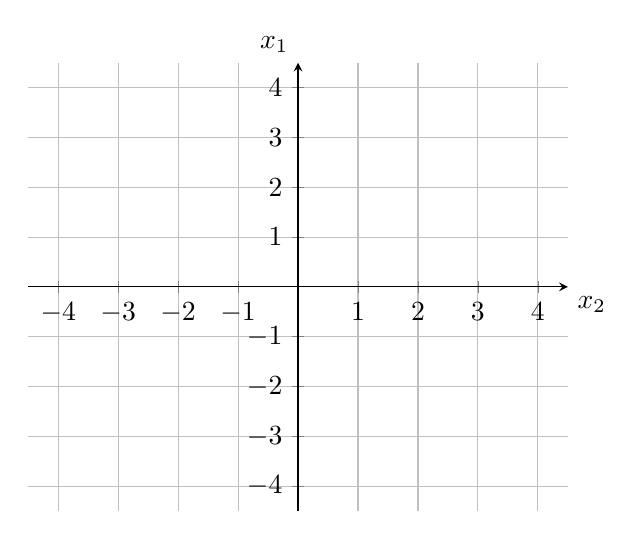
\begin{tikzpicture}[>=latex]
\begin{axis}[
  axis x line=center,
  axis y line=center,
   xtick={-4,...,4},
  ytick={-4,...,4},
  xlabel={$x_2$},
  ylabel={$x_1$},
  xlabel style={below right},
  ylabel style={above left},
  xmin=-4.5,
  xmax=4.5,
  ymin=-4.5,
  ymax=4.5,
  grid]
\end{axis}
\end{tikzpicture}
\end{center}

\begin{enumerate}
  \item Consider the vector $\vec{x} = \begin{bmatrix}2 \\ 4\end{bmatrix}$. Draw it on the graph provided. Also draw the vector $\vec{y_1} = \begin{bmatrix}1 \\ 0\end{bmatrix}$ and $\vec{y_2} = \begin{bmatrix}0 \\ 1\end{bmatrix}$. Now, find the projections of $\vec{x}$ on $\vec{y_1}$ and $\vec{y_2}$ geometrically. Compare with mathematical calculations.


\ans{

\begin{center}
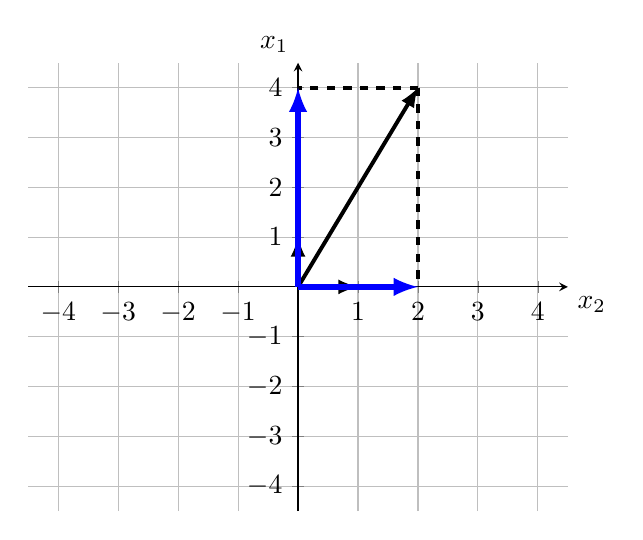
\begin{tikzpicture}[>=latex]
\begin{axis}[
  axis x line=center,
  axis y line=center,
   xtick={-4,...,4},
  ytick={-4,...,4},
  xlabel={$x_2$},
  ylabel={$x_1$},
  xlabel style={below right},
  ylabel style={above left},
  xmin=-4.5,
  xmax=4.5,
  ymin=-4.5,
  ymax=4.5,
  grid]
  \draw[->,line width=0.5mm] (axis cs:0,0) -- (axis cs:2,4);
  \draw[->, line width=0.5mm] (axis cs:0,0) -- (axis cs:1, 0);
  \draw[->, line width=0.5mm] (axis cs:0,0) -- (axis cs:0, 1);
  \draw[dashed, line width=0.5mm] (axis cs:2, 4) -- (axis cs:2,0);
  \draw[dashed, line width=0.5mm] (axis cs:2,4) -- (axis cs:0,4);
  \draw[->, line width=0.7mm, blue] (axis cs:0,0) -- (axis cs:2, 0);
  \draw[->, line width=0.7mm, blue] (axis cs:0,0) -- (axis cs:0, 4);
\end{axis}
\end{tikzpicture}
\end{center}

The projection of vector $\vec{b}$ on vector $\vec{a}$ is given by:
\begin{align}
\text{proj}_{\vec{a}} \vec{b}=\frac{\innp {\vec{b}}{\vec{a}}}          {\norm{\vec{a}}^2}\vec{a}
\end{align}
 Now we have:
$$\innp{\vec{x}}{\vec{y_1}} = 2 \cdot 1 + 4 \cdot 0 = 2$$
$$\innp{\vec{x}}{\vec{y_2}} = 2 \cdot 0 + 4 \cdot 1 = 4$$
$$\norm{\vec{y_1}}=\sqrt{1+0}=1$$
$$\norm{\vec{y_2}}=\sqrt{0+1}=1$$
Hence projection of vector $\vec{x}$ on vector $\vec{y_1}$ is
\begin{align}
\text{proj}_{\vec{y_1}} \vec{x}=\frac{\innp {\vec{x}}{\vec{y_1}}}{\norm{\vec{y_1}}^2}\vec{y_1}=\frac{2}{1}\begin{bmatrix}1 \\ 0\end{bmatrix}=\begin{bmatrix}2 \\ 0\end{bmatrix}\\
\text{proj}_{\vec{y_2}} \vec{x}=\frac{\innp {\vec{x}}{\vec{y_2}}}{\norm{\vec{y_2}}^2}\vec{y_2}=\frac{4}{1}\begin{bmatrix}0 \\ 1\end{bmatrix}=\begin{bmatrix}0 \\ 4\end{bmatrix}
\end{align}

}


\item Calculate the projection of $\vec{x}=\begin{bmatrix}1 \\ 1\end{bmatrix}$ on $\vec{y}=\begin{bmatrix}3 \\ 4\end{bmatrix}$. Is it the same as the projection of $\vec{y}$ on $\vec{x}$?

\meta{
Highlight that the order of the vectors matters in the expression of projection.
}
\ans{
Hence projection of vector $\vec{x}$ on vector $\vec{y}$ is
\begin{align}
\text{proj}_{\vec{y}} \vec{x}=\frac{\innp {\vec{x}}{\vec{y}}}{\norm{\vec{y}}^2}\vec{y}=\frac{1\cdot3+1\cdot4}{3^2+4^2}\begin{bmatrix}3 \\ 4\end{bmatrix}=\frac{7}{25}\begin{bmatrix}3 \\ 4\end{bmatrix}.
\end{align}
Now the projection of vector $\vec{y}$ on vector $\vec{x}$ is given by
\begin{align}
\text{proj}_{\vec{x}} \vec{y}=\frac{\innp {\vec{y}}{\vec{x}}}{\norm{\vec{x}}^2}\vec{x}=\frac{3\cdot1+4\cdot1}{1^2+1^2}\begin{bmatrix}1 \\ 1\end{bmatrix}=\frac{7}{2}\begin{bmatrix}1 \\ 1\end{bmatrix}=\begin{bmatrix}3.5 \\ 3.5\end{bmatrix},
\end{align}
which is not the same as $\text{proj}_{\vec{x}} \vec{y}$.
}

\item Now consider the vectors $\vec{x} = \begin{bmatrix}1\\ 2 \\ 4\end{bmatrix}$,  $\vec{y_1} = \begin{bmatrix}1 \\ 1 \\ 0\end{bmatrix}$ and $\vec{y_2} = \begin{bmatrix}0 \\ 0\\ 1\end{bmatrix}$. Now, find the projections of $\vec{x}$ on $\vec{y_1}$ and $\vec{y_2}$. Also find the projection of $\vec{x}$ on $\text{span}\{\vec{y_1}, \vec{y_2}\}$. 
Is $\text{proj}_{\vec{y_1}} \vec{x}+\text{proj}_{\vec{y_2}} \vec{x}$ equal to $\text{proj}_{\text{span}\{\vec{y_1}, \vec{y_2}\}} \vec{x}$? Explain your answer.


\meta{
\begin{itemize}
\item Make sure to note that the summation of projections on orthogonal vectors will be the same as the projection on the subspace spanned by those orthogonal vectors. This is only true for orthogonal vectors.
\item Also mention that it is not useful to visualize the vector with higher dimensions than 3.
\end{itemize}

}

\ans{
The projection of vector $\vec{x}$ on vector $\vec{y_1}$ is
\begin{align}
\text{proj}_{\vec{y_1}} \vec{x}=\frac{\innp {\vec{x}}{\vec{y_1}}}{\norm{\vec{y_1}}^2}\vec{y_1}=\frac{1\cdot1+2\cdot1++4\cdot0}{1^2+1^2+0^2}\begin{bmatrix}1 \\ 1 \\ 0\end{bmatrix}=\frac{3}{2}\begin{bmatrix}1 \\ 1 \\ 0\end{bmatrix}=\begin{bmatrix}1.5 \\ 1.5 \\ 0\end{bmatrix}.
\end{align}
Similarly projection of vector $\vec{x}$ on vector $\vec{y_2}$ is
\begin{align}
\text{proj}_{\vec{y_2}} \vec{x}=\frac{\innp {\vec{x}}{\vec{y_2}}}{\norm{\vec{y_2}}^2}\vec{y_2}=\frac{1\cdot0+2\cdot0++4\cdot1}{0^2+0^2+1^2}\begin{bmatrix}0 \\ 0\\ 1\end{bmatrix}=\frac{4}{1}\begin{bmatrix}0 \\ 0\\ 1\end{bmatrix}=\begin{bmatrix}0 \\ 0\\ 4\end{bmatrix}.
\end{align}
We can use the least squares formula to find the projection of a vector on a subspace. The the projection of $\vec{x}$ on $\text{span}\{\vec{y_1}, \vec{y_2}\}$ is the same as projection of $\vec{x}$ on $\text{col}\{\mathbf{A}\}$, where matrix $\mathbf{A}$ has the columns $\vec{y_1}$ and $\vec{y_2}$.
\begin{align}
\text{proj}_{\text{span}\{\vec{y_1}, \vec{y_2}\}} \vec{x}=\mathbf{A}\hat{\vec{\alpha}}=\mathbf{A}(\mathbf{A}^T\mathbf{A})^{-1}\mathbf{A}^T\vec{x}, 
\end{align}
where $\hat{\vec{\alpha}}$ is the least squares solution to $\mathbf{A}\vec{\alpha}=\vec{x}$.

Now we can calculate:
$$\mathbf{A}^T\mathbf{A}=\begin{bmatrix}
1 & 1 & 0\\ 0 & 0 & 1
\end{bmatrix}\begin{bmatrix}
1 & 0\\ 1 & 0\\ 0& 1
\end{bmatrix}=\begin{bmatrix}
2 & 0\\ 0& 1
\end{bmatrix}$$
$$(\mathbf{A}^T\mathbf{A})^{-1}=\begin{bmatrix}
0.5 & 0\\ 0& 1
\end{bmatrix}$$
$$\mathbf{A}^T\vec{x}=\begin{bmatrix}
1 & 1 & 0\\ 0 & 0 & 1
\end{bmatrix}\begin{bmatrix}1\\ 2 \\ 4\end{bmatrix}=\begin{bmatrix}3 \\ 4\end{bmatrix}$$
So we can calculate
$$\text{proj}_{\text{span}\{\vec{y_1}, \vec{y_2}\}} \vec{x}=\mathbf{A}(\mathbf{A}^T\mathbf{A})^{-1}\mathbf{A}^T\vec{x}=\begin{bmatrix}
1 & 0\\ 1 & 0\\ 0& 1
\end{bmatrix}\begin{bmatrix}
0.5 & 0\\ 0& 1
\end{bmatrix}\begin{bmatrix}3 \\ 4\end{bmatrix}=\begin{bmatrix}
1 & 0\\ 1 & 0\\ 0& 1
\end{bmatrix}\begin{bmatrix}1.5 \\ 4\end{bmatrix}=\begin{bmatrix}1.5 \\ 1.5\\ 4\end{bmatrix}$$.

Now summing up the projections on $\vec{y_1}$ and $\vec{y_2}$, we have 
$$\text{proj}_{\vec{y_1}} \vec{x}+\text{proj}_{\vec{y_2}} \vec{x}=\begin{bmatrix}1.5 \\ 1.5 \\ 0\end{bmatrix}+\begin{bmatrix}0 \\ 0\\ 4\end{bmatrix}=\begin{bmatrix}1.5 \\ 1.5 \\ 4\end{bmatrix}=\text{proj}_{\text{span}\{\vec{y_1}, \vec{y_2}\}}$$.
Here $\text{proj}_{\vec{y_1}} \vec{x}+\text{proj}_{\vec{y_2}} \vec{x}$ is equal to $\text{proj}_{\text{span}\{\vec{y_1}, \vec{y_2}\}} \vec{x}$ since $\vec{y_1}$ and $\vec{y_2}$ are orthogonal, i.e. $\innp{\vec{y_1}}{\vec{y_2}}=0$.
}

\item{
Find the expression for projection of $\vec{b}=\begin{bmatrix}1 \\ 2 \\ 4\end{bmatrix}$ on the columnspace of matrix $\mathbf{A}=\begin{bmatrix}| & | \\ \vec{a_1} & \vec{a_2} \\ | & |\end{bmatrix}=\begin{bmatrix}1 & 1 \\ 1 & 0 \\ 1 & 0\end{bmatrix}$. 

Is $\text{proj}_{\vec{a_1}} \vec{b}+\text{proj}_{\vec{a_2}} \vec{b}$ equal to $\text{proj}_{\text{Col}\{\mathbf{A}\}} \vec{b}$? (No need to do the calculations.)

If we set up a system of linear equations $\mathbf{A}\vec{x}=\vec{b}$, will there be a unique solution? (No need to solve the system.) 

}

\meta{
Reminder: that we can always get a solution from least squares, even if it's not unique. (Highlighting that the uniqueness of the solutions depends on the invertibility of A).
}

\ans{
We use the least squares formula again to find the projection of a vector on a subspace. The the projection of $\vec{b}$ on $\text{Col}\{\mathbf{A}\}$ is
\begin{align}
\text{proj}_{\text{Col}\{\mathbf{A}\}} \vec{b}=\mathbf{A}\hat{\vec{\x}}=\mathbf{A}(\mathbf{A}^T\mathbf{A})^{-1}\mathbf{A}^T\vec{b}, 
\end{align}
where $\hat{\vec{\x}}$ is the least squares solution to $\mathbf{A}\vec{\x}=\vec{b}$.

Now we can calculate:
$$\mathbf{A}^T\mathbf{A}=\begin{bmatrix}
1 & 1 & 1\\ 1 & 0 & 0
\end{bmatrix} \begin{bmatrix}1 & 1 \\ 1 & 0 \\ 1 & 0\end{bmatrix} =\begin{bmatrix}
3 & 1\\ 1 & 1
\end{bmatrix}$$
$$(\mathbf{A}^T\mathbf{A})^{-1}=\begin{bmatrix}
0.5 & -0.5\\ -0.5 & 1.5
\end{bmatrix}$$
$$\mathbf{A}^T\vec{x}=\begin{bmatrix}
1 & 1 & 1\\ 1 & 0 & 0
\end{bmatrix}\begin{bmatrix}1\\ 2 \\ 4\end{bmatrix}=\begin{bmatrix}7 \\ 1\end{bmatrix}$$
So we can calculate
$$\text{proj}_{\text{Col}\{\mathbf{A}\}}\vec{b} =\mathbf{A}(\mathbf{A}^T\mathbf{A})^{-1}\mathbf{A}^T\vec{b}=\begin{bmatrix}
1 & 1\\ 1 & 0\\ 1& 0
\end{bmatrix}\begin{bmatrix}
0.5 & -0.5\\ -0.5& 1.5
\end{bmatrix}\begin{bmatrix}7 \\ 1\end{bmatrix}=\begin{bmatrix}
0 & 1\\ 0.5 & -0.5\\ 0.5 & -0.5
\end{bmatrix}\begin{bmatrix}7 \\ 1\end{bmatrix}=\begin{bmatrix}1 \\ 3\\ 3\end{bmatrix}.$$

The columns of $\mathbf{A}$ are not orthogonal, so $\text{proj}_{\vec{a_1}} \vec{b}+\text{proj}_{\vec{a_2}} \vec{b}$ is not equal to $\text{proj}_{\text{Col}\{\mathbf{A}\}} \vec{b}$.

There won't be a unique solution to $\mathbf{A}\vec{x}=\vec{b}$, since $\text{proj}_{\text{Col}\{\mathbf{A}\}} \vec{b}\neq \vec{b}$. This means that $\vec{b}$ is not in the columnspace of $\mathbf{A}$, so the system is inconsistent.
}

\end{enumerate}
